\documentclass[a4paper]{article}

% Because it looks better:
\usepackage{a4wide}
% Take care of input things:
\usepackage[utf8]{inputenc}
\usepackage[T1]{fontenc}
% Packages for pictures:
\usepackage{graphicx}
\usepackage{float}
\usepackage{listings}
\lstset{numbers=left, numberstyle=\tiny, numbersep=5pt}
\lstset{language=Perl}
% Package for urls:
\usepackage{url}

\bibliographystyle{alpha}

% Now let us define a few shortcuts:
% Correct sign for C#:
\newcommand{\CS}{C\nolinebreak\hspace{-.05em}\raisebox{.6ex}{\scriptsize\bf \#\ }}

% --------------------------------------------------------------------------------------------!
%
% NOTE: For better usage of LaTeX with GIT, please write each sentence on an own line, separating paragraphs
%       by the usual double returns. That way GIT can track each sentence on its own instead of always
%       having to track a paragraph as one block.
%
% --------------------------------------------------------------------------------------------!

\begin{document}

\title{Documentation}
\author{Andreas Köll, Johannes Bohner, Burkhard Hoppenstedt, Tamino Hartmann}
\date{\today}

\maketitle

\begin{abstract}

Abstract here
\end{abstract}
\newpage

\section{Introduction}

This paper represents a rework of \cite{origin}.
We analyzed what the authors did and tried the method on a somewhat different study.
Here we show the documentation to our work, our conclusions, and how our work compares to the original work.

\section{Setup of the Experiment}

This section describes the way the data was recorded to the best of our abilities.
We'll first look at the hardware and software side of things and then continue on to the actual proceedings that were established to capture the motion data required for the analysis.

\subsection{Equipment}

For our recording we used the "Kinect for Windows"\texttrademark \cite{kinect}, connected to a computer running "Microsoft Windows 7"\textregistered \ via USB.
The Kinect is mounted on a tripod to allow correct positioning.
The weights were applied with a weight-vest with a weight of 5 kilograms.
For the alternate motion, skipping, we also provided a rope.
We used normal tape to mark positions on the floor so that all recordings were made with the same measurements.

\subsection{Software}

We developed our own application for recording the input stream from the Kinect in \CS with "Microsoft Visual Studio 2012" utilizing the "Microsoft Kinect Developer Version".
The program is currently available as open source here \cite{csprogram} and can be seen in Fig ~\ref{fig:programm}.

\begin{figure}[H]
	\centering
	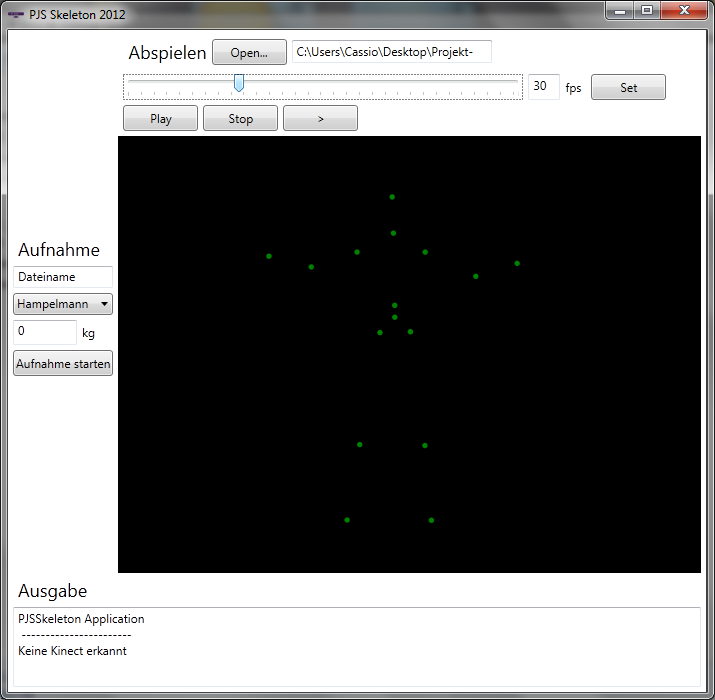
\includegraphics[width=8cm]{programm.jpg}
	\caption{Screenshot of the program used to record the data.}
	\label{fig:programm}
\end{figure}

Later steps that were based on the recorded data were programmed in MATLAB, available here \cite{matlabprograms}.

\subsection{Workflow}

As the overall workflow of the data from its capture to final results is non-trivial, we have provided a flowchart of the procedure to help understand what code does what when and which data files represent what intermediate results\footnote{TODO: Add flowchart here!}.

\subsection{Composition of the Recording}

Figure \ref{fig:schematic} shows the schematics of the arrangement of the Kinect for the recordings\footnote{TODO: Change figure to have english text!}.
The way the Kinect records skeletons proved to be a strong limiting factor in selecting which motions to record as the depth-perception is comparatively poor.
The fixed nature of the experiment also limited the motion to one that could be done within a small area, which disclosed for example any form of walking or running.

\begin{figure}
	\centering
	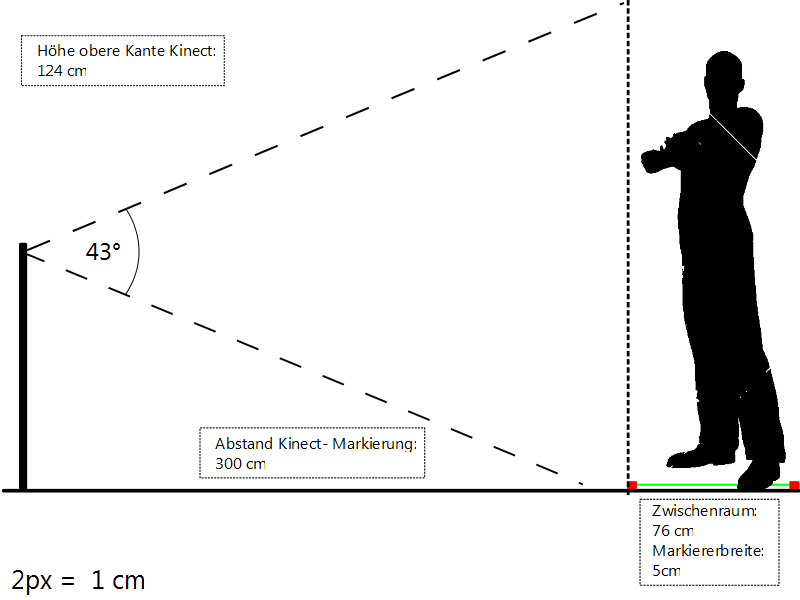
\includegraphics[width=10cm]{Aufbau.png}
	\caption{Schematics of the arrangement for the recording of our source data.}
	\label{fig:schematic}
\end{figure}

\section{Visualisation}

This section is independent from the rest of the paper as the analytical methods don't matter. Out intent is to show the captured points of the skeleton in an representative 3D Model.

\subsection{Absolute vs. Relative Values}
As seen in the description of storing points in a ".txt" file the kinect uses Absolute Values to represent the skeleton  - which is absolutely useful, because otherwise it couldn't detect different lengths in body parts. Instead it would had to map the measured values on a defined body model. This procedure would cause inaccuracy.\
While animating a defined model in the opposite you can't just easily scale single body parts to adjust the proportions. This problem needs as a solution a format invariant to scaling.

\subsection{The .bvh file}
\begin{lstlisting}[caption=.bvh Connected Structure]{Name}
JOINT lCollar
{
		OFFSET	1.858774 10.237258 -1.915852
		CHANNELS 3 Zrotation Yrotation Xrotation
		JOINT lShldr
		{
			OFFSET	6.103279 0.000102 -0.038601
			CHANNELS 3 Zrotation Yrotation Xrotation
			JOINT lForeArm
\end{lstlisting}

\end{document}

\section{Conclusion}

TODO: Put conclusion here.

\newpage
\bibliography{doc}

\end{document}